\documentclass{article}
\usepackage{indentfirst}
\usepackage{graphicx}
\usepackage{array}

\title{Shortcut to Knowledge: Answering Questions About Horse Racing with Data}
\author{Jack Karisch}
\date{June 2021}


\begin{document}

\begin{figure}
    \centering
    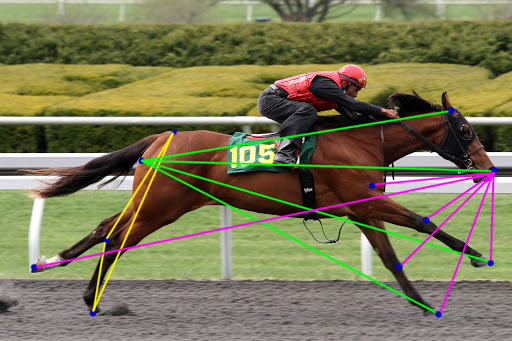
\includegraphics[width=12cm]{images/horse_data_image.png}
\end{figure}

\maketitle

This paper documents my attempt to learn as much as possible about thoroughbred racing by using data. My goal is to find a shortcut to the kind of knowledge veteran horseplayers accrue after years around the sport in a fraction of the time. The data is taken from Equibase results for all races run between January 1, 2020 and June 30, 2021. Each section will be a response to a basic question prompt that a curious spectator might ask about the sport. This paper will expand over time as I answer more of these questions.

\section*{How accurate are the odds?}

This is the most basic question a first-time bettor would ask. Like a stock price, the odds dictate the opinion of the market. In a system with perfect information, they would precisely predict the order of finish of every race. This obviously isn't the case, but how close do they get?

\begin{figure}
    \centering
    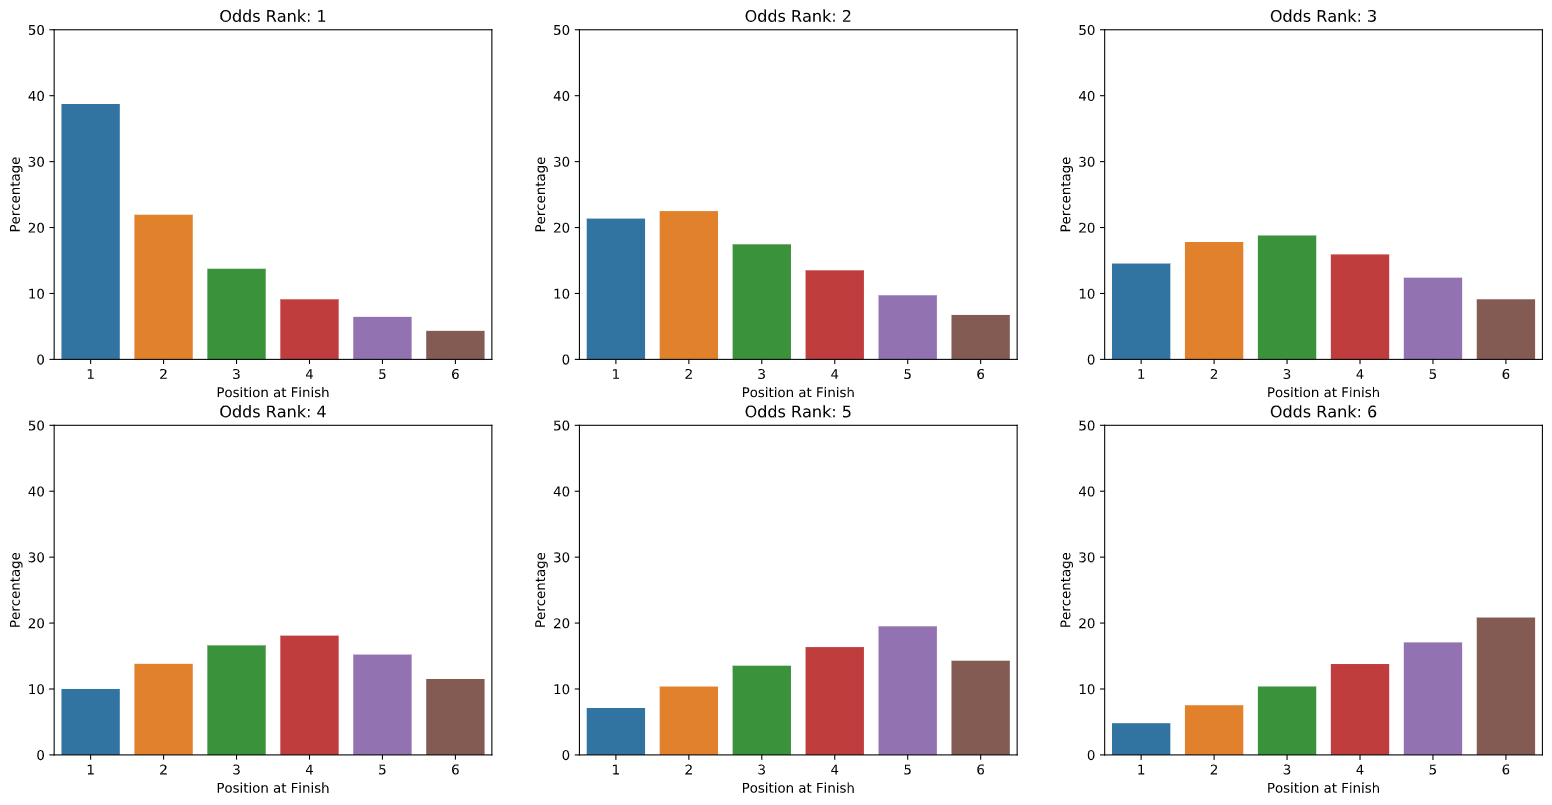
\includegraphics[width=12cm]{images/odds_rank_finish_chart.png}\medskip

    \caption{Percentage of runs finishing in position 1-6 for six favorites}
    \label{figure:oddsRanksFinish}

\end{figure}

Figure \ref{figure:oddsRanksFinish} provides a very basic answer to this question. The favorite won in 39\% of races, placed in 61\% and showed in 74\%. The second favorite placed in 44\% of races and showed in 63\%. The third favorite showed 51\% of the time. In general, the odds do predict the order of finish (at least through the first 6 positions), but with a lot of uncertainty. The odds predict the winner with much more success than they predict any other finisher, which makes sense because that's exactly what bettors are trying to do; it makes no difference to a gambler if his horse finishes second or dead last if he places a win bet.

\begin{figure}
    \centering
    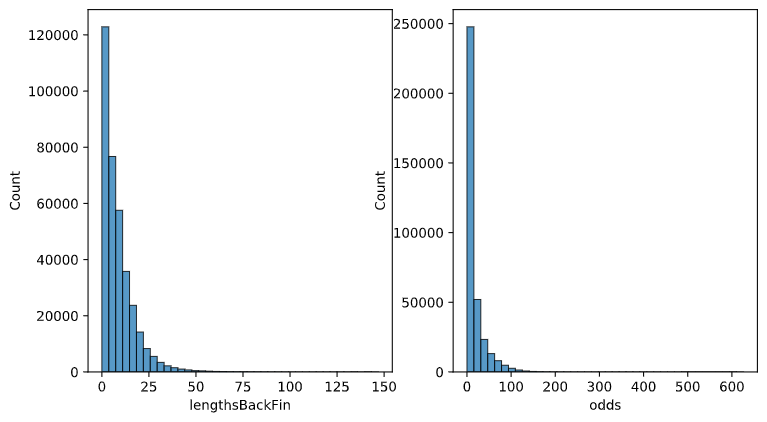
\includegraphics[width=12cm]{images/lengths_odds_no_trans_chart.png}

    \caption{Distribution of raw odds and lengths back variables} 
    \label{figure:oddsLengthsNoTrans} 
\end{figure}

In order to check whether the odds can predict the relative performance of the horses, we turn to linear regression. The goal is to find the effect of increasing odds on the number of lengths back from the leader a horse finishes. Figure \ref{figure:oddsLengthsNoTrans} shows the distribution of the variables encoding odds and number of lengths behind leader at the finish of the race. Both of these distributions show aggressive right skew, so they are poor candidates for a linear regression fit in their. One reason the lengths back variable shows this pattern could be because horse racing is constructed in such a way that all the horses finish as closely as possible to one another (for example, better horses generally have to carry more weight). The odds variable follows the pattern because of the nature of picking a favorite. Most races will have at least one horse in the 0-2 range for odds, but relatively few will have one in the 20-22 range, and even fewer in the 60+ range. This is shown in Figure \ref{figure:oddsRankMeansStds}. The standard deviation is tighter for lower odds, leading to more observations close together on the left end of the distribution.

Both variables can be transformed to distributions closer to normal; taking the lengths deviation from average in the race for each horse gives the distribution in the left plot of Figure \ref{figure:oddsLengthsYesTrans}, taking the 8th root of odds gives the distribution shown in the middle of Figure \ref{figure:oddsLengthsYesTrans}. A scatter plot (including the linear regression line) of the transformed variables is shown on the right. 

The output of a linear regression of the transformed lengths variable on the transformed odds variable, using a random sample of 5000 horses:

\begin{figure}[h]
    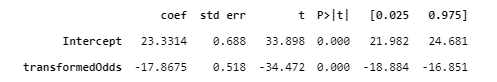
\includegraphics[width=12cm]{images/odds_lengths_regression.png}   
\end{figure}

\begin{figure}
    \centering
    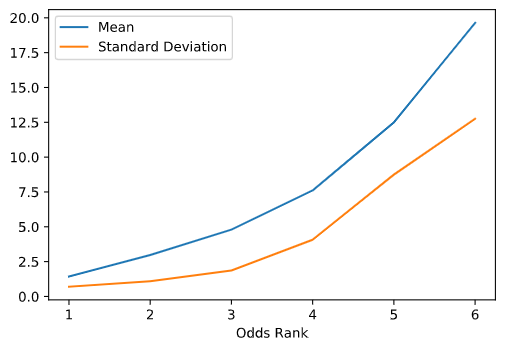
\includegraphics[width=8cm]{images/odds_rank_means_stds.png}

    \caption{Mean and standard deviation for six favorites} 
    \label{figure:oddsRankMeansStds}   
\end{figure}

\begin{figure}
    \centering
    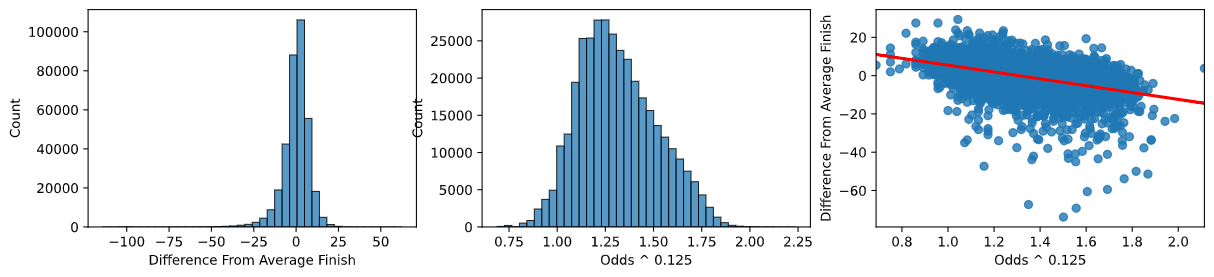
\includegraphics[width=13cm]{images/lengths_odds_yes_trans_chart.png}

    \caption{Transformed odds and lengths back variables}
    \label{figure:oddsLengthsYesTrans}
\end{figure}

\noindent This regression suggests that odds are strongly predictive of the margin of finish, relative to a good amount of variability. Interpretation is somewhat difficult because of the transformations; basically, every unit increase in the eighth root of the odds of a particular horse adds ~18 lengths to the finishing position of that horse. To aid with intuition, the expected lengths relative to average for a range of untransformed odds can be found in Figure \ref{figure:oddsLengthsRegActual}. 

\begin{figure}
    \centering
    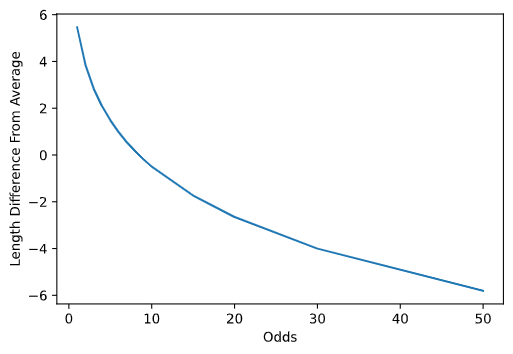
\includegraphics[width=8cm]{images/odds_lengths_actual_reg_chart.png}

    \caption{Lengths relative to average at finish for odds from 1-50} 
    \label{figure:oddsLengthsRegActual}   
\end{figure}

\section*{What are the payouts of basic betting strategies?}

First, the term "basic betting strategies" needs to be defined. In answering this question, the following strategies will be considered: always betting on the favorite to win, always betting on the second favorite to place, always betting on the third favorite to show, always betting on the first and second favorite in that order for an exacta, and always betting on the first three favorites in that order for a trifecta. The results appear in the table below. These results assume that a \$2 bet was placed on every race in which betting of the type in question was allowed for all the races in the dataset.

\begin{center}
    \begin{tabular}{ |l|c|c|c| } 
     \hline
     \textbf{Strategy} & \textbf{Wagered} & \textbf{Won} & \textbf{Net} \\
     \hline
     Favorite to win & \$90,710 & \$79,658 & -\$11,052 \\ 
     \hline
     2nd favorite to place & \$90,144 & \$98,560 & \$8,446 \\ 
     \hline
     3rd favorite to show & \$84,776 & \$84,075 & -\$701 \\ 
     \hline
     Top 2 favorites exacta & \$88,068 & \$75,376 & -\$12,692 \\ 
     \hline
     Top 3 favorites trifecta & \$86,802 & \$70,191 & -\$16,611 \\
     \hline
    \end{tabular}
\end{center}

Unsurprisingly, most of these strategies result in net losses. Assuming no track take (the amount of the total wagered the track skims for each race, generally around 15\% for win/place/show pools), more of these could porentially be viable, but horse betting is not the kind of game where winning 51\% means making money; it's probably closer to 60\% or even 65\%. Regardless, the only real surprise here is the success of the second favorite to place strategy, which resulted in a respectable return of 9\%. Would this return hold up long term? Probably not, since it's a very simple technique that would occur to even first-time bettors, and if its expected value were positive long term it would be exploited by more experienced players. However, it's a good baseline bet to place if further analysis is infeasible.

\section*{What is the breakdown of win/place/show wagering?}

Unfortunately, the Equibase results charts that the data is pulled from do not track much info about place and show bets. They give a figure for the total WPS (win/place/show) pool, as well as the odds to win for each horse.

\section*{?}

\end{document}